\section{Данные}
Датасета для обучения моделей для извлечения атрибутов пока не существует. Из-за этого, в данной работе взаимствован датасет GTKY из статьи \cite{gtky}. Он создан методом distant supervision из датасета DialogueNLI \cite{dnli}, который в свою очередь построен на основе датасета PersonaChat \cite{personachat}. Ниже будет дан краткий обзор каждого из датасетов.

\textbf{PersonaChat}    Датасет содержащий примерно 10.000 диалогов открытого домена, в среднем состоящие из 10-15 реплик. Имеется разметкая каждого диалога по персонам собеседников. Пример диалога можно увидеть на Рисунке \ref{fig:pc_sample}. В датасете насчитывается 1155 персон с 5000 предложениями в неструктурированном формате на естественном языке, которые идут перед диалогами, но при этом, нет четкого соответствия между предложениями персоны и репликами.

\textbf{DialogueNLI}    Относительно новый датасет для NLI задач (\cite{nli_survey}) в диалоговом домене, построенный над датасетом PersonaChat. Состоит из пар реплик с метками импликации, нейтральности и противоречия (entailment, neutral, contradiction). Например, на Рисунке \ref{fig:pc_sample} реплика Персоны А "I just got back from the club." является следствием предложения "I like to dance at the club.". Каждое предложение персоны в датасете имеет разметку в виде триплета \textit{(subject, relation, object)}, в котором \textit{relation} - это отношение из предопределенного множества отношений, например \textit{live\textunderscore in\textunderscore general}, \textit{like\textunderscore goto}, \textit{have\textunderscore pet}. В датасете DialogueNLI таких отношений 61, и все множество этих отношений можно найти в приложениях к статье \cite{dnli}. C примерной структурой датасета можно ознакомиться на Рисунке \ref{fig:dnli_sample}.

\textbf{GTKY}   Так как в датасете DialogueNLI не все реплики имеют разметку по триплетам, авторы статьи \cite{gtky} применили SOTA NLI модель, чтобы соотнести предложения персон к репликам. То есть, если предложение персоны и реплика имеют положительный entailment, то какой то атрибут из этой реплики представляется в виде триплета соответствующего этому предложению персоны. Например, реплика "I prefer basketbal; team sports are fun." и предложение "I like playing basketball." имеют положительный entailment, поэтому данной реплике можно присвоить триплет персоны \textit{(I, like\textunderscore sports, basketball)} в качестве одного из атрибутов. В качестве NLI модели для определения степени entailment'a двух предложений был использован BERT \cite{devlin_bert}, дообученный на датасете DialogueNLI, который получил точность 88.43\% на тестовой выборке.

\subsection{Анализ датасета GTKY}

Размеры обучающей, тестовой и валидационной выборки равны 131.424, 15.008 и 15.586 соответственно. Cо статистиками по распределению количества триплетов по репликам можно ознакомиться в Таблице \ref{table:triple_count_stats} и на Рисунке \ref{fig:triple_distr}. Как можно увидеть, в датасете около 50\% примеров имеют пустой целевой набор атрибутов. Так же можно посмотреть на распределение типов отношений на Рисунке \ref{fig:predicate_distr}, а самые часто и самые редко встречающиеся сущности показаны в Таблице \ref{table:top5_subj} и \ref{table:top5_obj}.

Техника distant supervision заменяет человеческую разметку данных, однако, вводит другие трудности, представленные шумом в данных что видно в Таблице \ref{table:gtky_noise}.
 
\begin{figure}[!ht]
    \centering
    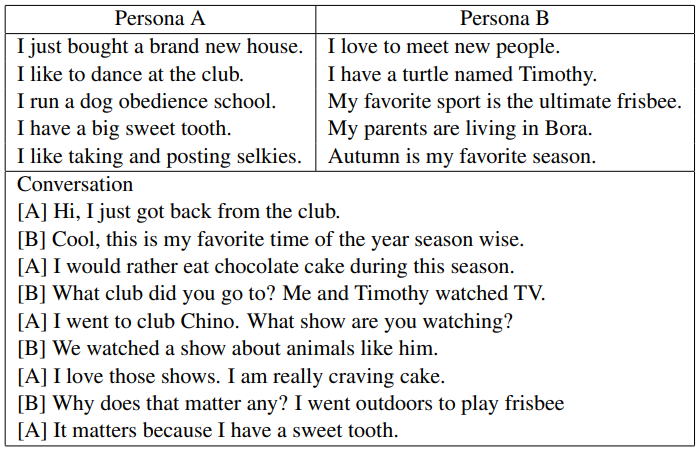
\includegraphics[width=0.8\textwidth]{images/pc_example.png}
    \caption{Пример диалога из датасета PersonaChat. Персоны собеседников заданы перед диалогом.}
    \label{fig:pc_sample}
\end{figure}

\begin{figure}[!ht]
    \centering
    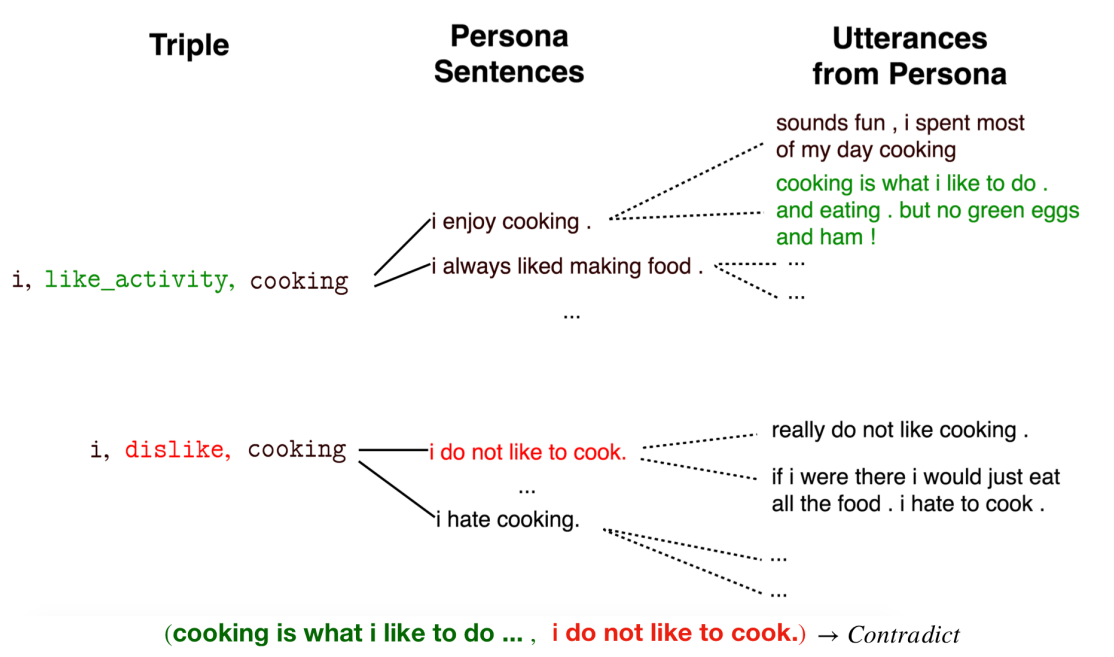
\includegraphics[width=0.8\textwidth]{images/dnli_example.png}
    \caption{Пример из датасета DialogueNLI и схема соотношения триплетов к репликам.}
    \label{fig:dnli_sample}
\end{figure}

\begin{table}[!ht]
\centering
\begin{tabular}{c|c c c}
    \hline
     & TRAIN & TEST & VALIDATION \\
    \hline
    \hline
    \textbf{max} & 6 & 5 & 5 \\
    \hline
    \textbf{mean} & 0.61 & 0.61 & 0.63 \\
    \hline
    \textbf{median} & 0 & 0 & 1 \\
    \hline
\end{tabular}
\caption{Статистики количества триплетов в репликах в датасете GTKY.}
\label{table:triple_count_stats}
\end{table}

\begin{figure}[!ht]
    \centering
    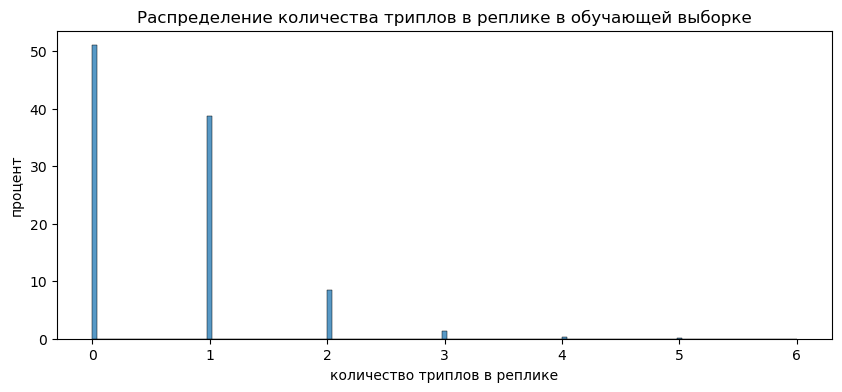
\includegraphics[width=0.9\textwidth]{images/triple_distr_train.png}
    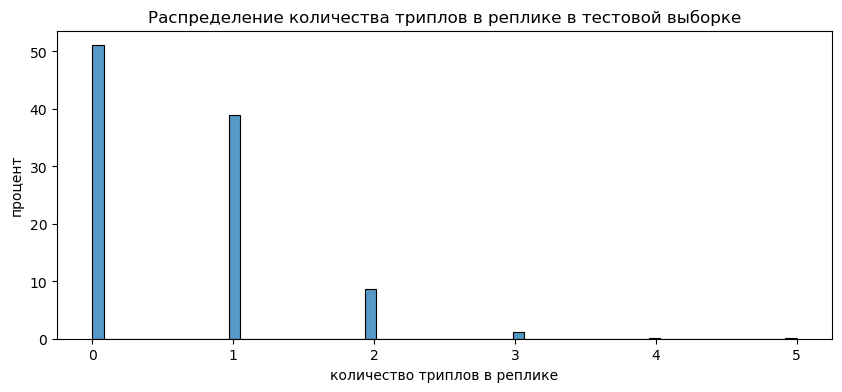
\includegraphics[width=0.9\textwidth]{images/triple_distr_test.png}
    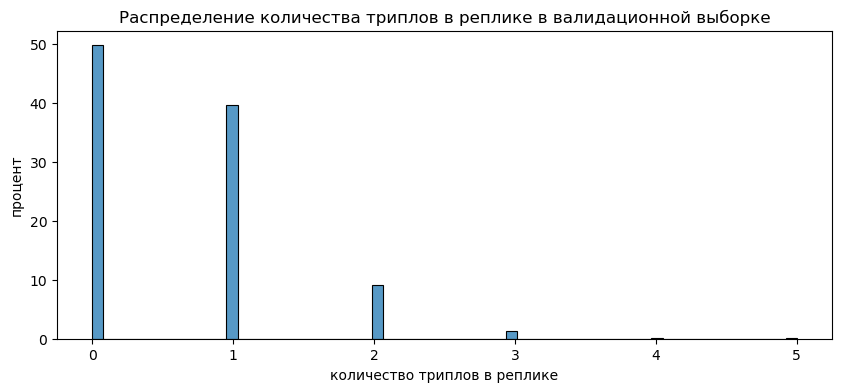
\includegraphics[width=0.9\textwidth]{images/triple_distr_val.png}
    \caption{Распределения количества триплетов в репликах в разных выборках датасета GTKY.}
    \label{fig:triple_distr}
\end{figure}

\begin{figure}[!ht]
    \centering
    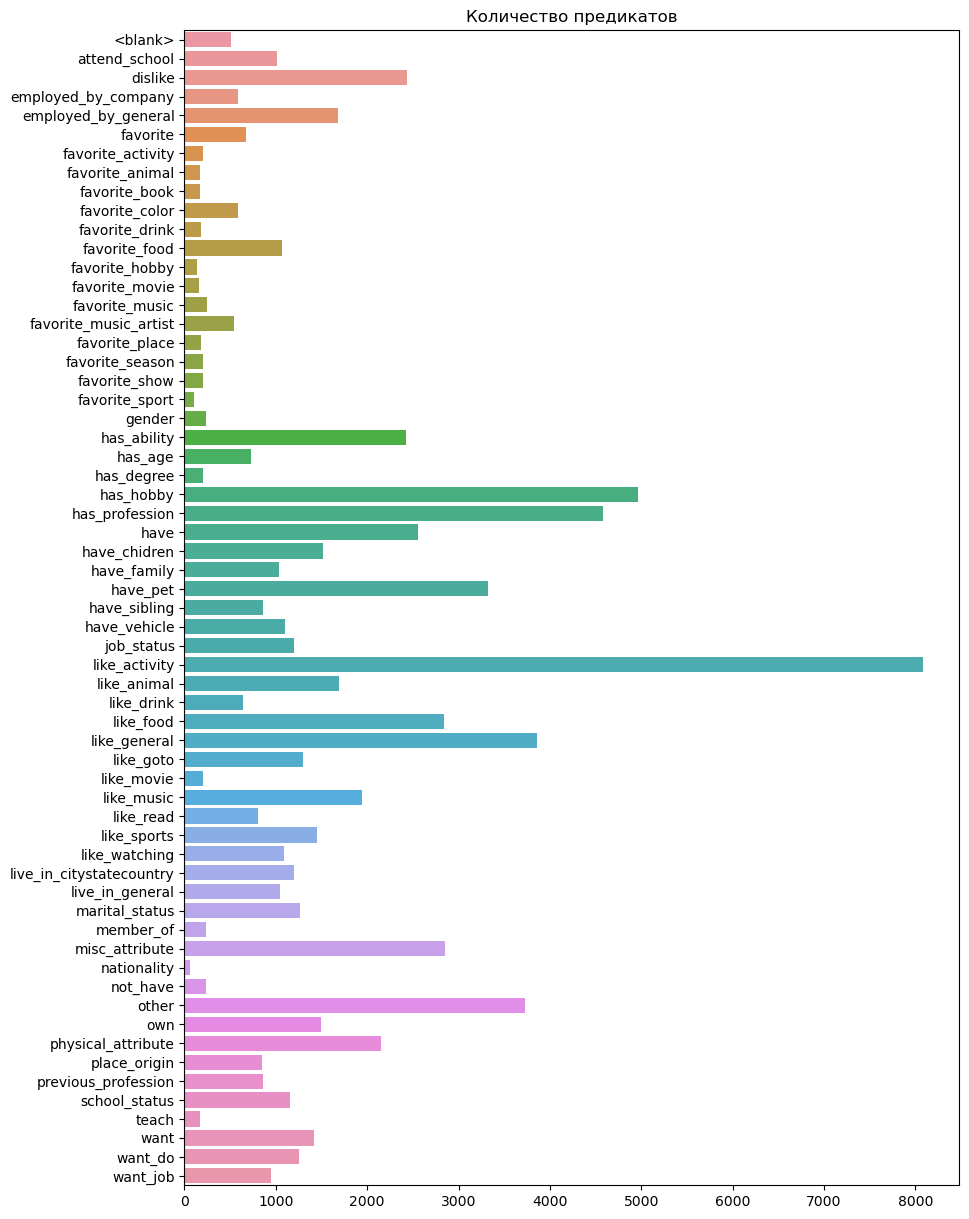
\includegraphics[width=0.95\textwidth]{images/predicate_distr.png}
    \caption{Распределение типов отношений в обучающей выборке датасета GTKY.}
    \label{fig:predicate_distr}
\end{figure}

\begin{table}[!ht]
\centering
\begin{tabular}{|c|c|}
    \hline
     Субъект & Количество \\
     \hline
    i & 75202 \\
    \hline
    my mother & 988 \\
    \hline
    my & 567 \\
    \hline
    my brother & 204 \\
    \hline
    my parents & 203 \\
    \hline
    \hline
    my career & 1 \\
    \hline
    my marriage & 1 \\
    \hline
    commitment & 1 \\
    \hline
    my foster & 1 \\
    \hline
    dude & 1 \\
    \hline
\end{tabular}
\caption{Топ-5 самых часто и редко встречаемых субъектов среди триплетов в обучающей выборке датасета GTKY.}
\label{table:top5_subj}
\end{table}

\begin{table}[!ht]
\centering
\begin{tabular}{|c|c|}
    \hline
     Объект & Количество \\
     \hline
    dog & 1530 \\
    \hline
    \texttt{<blank>} & 1336 \\
    \hline
    cat & 992 \\
    \hline
    student & 760 \\
    \hline
    cooking & 723 \\
    \hline
    \hline
    hard time & 1 \\
    \hline
    5 pets & 1 \\
    \hline
    carriage & 1 \\
    \hline
    group & 1 \\
    \hline
    significant other & 1 \\
    \hline
\end{tabular}
\caption{Топ-5 самых часто и редко встречаемых объектов среди триплетов в обучающей выборке датасета GTKY.}
\label{table:top5_obj}
\end{table}

\begin{table}[!ht]
% \centering
\begin{tabular}{|m{15em}|m{15em}|}
    \hline
     Реплика & триплет \\
     \hline
     \hline
    all i can think about is moving away. & \textit{(my, like\textunderscore goto, desert)} \\
    \hline
    i have a wife i am in my early 40s. & \textit{()} \\
    \hline
    she is a golden retriever very nice dogs. & \textit{(my dog, other, name wonwon)} \\
    \hline
    i like to meet new people. & \textit{(i, live\textunderscore in\textunderscore citystatecountry, new york)} \\
    \hline
    i already mentioned them. but i like to spend time with my family and dogs. & \textit{()} \\
    \hline
    do you work anywhere ? i have a part time job. & \textit{()} \\
    \hline
    sounds like some awesome films. & \textit{(i, like\textunderscore goto, movie theater)} \\
    \hline
    rather get to know you i got free hp computer today. & \textit{(my adopted father, employed\textunderscore by\textunderscore company, hp)} \\
    \hline
\end{tabular}
\caption{Шум в разметке датасета GTKY с distant supervision.}
\label{table:gtky_noise}
\end{table}
